% !TEX root = RKWard_paper.tex
\section{Background and motivation}
\label{background}
In mid 1993 Ihaka and Gentleman published initial efforts on the computing
language and programming environment \proglang{R} on the \emph{s-news} mailing list. Ambitions for
this project were to develop an \proglang{S}-like language without inheriting memory
and performance issues. The source code of \proglang{R} was finally released in 1995, and
since 1997 development has evolved under the umbrella of the \proglang{R}
Development Core Team \citep{RDCT2001, RDCT2010, Ihaka_Gentlemen_1993}.
\proglang{R} does not include an advanced cross-platform GUI (graphical user interface) as known from other
statistical software packages. However, \proglang{R} includes tools for building GUIs
mainly based on \proglang{Tlc/Tk} \citep{Dalgaard2001, Dalgaard2002}. Since then a
plethora of \proglang{R} GUIs have emerged (see \url{http://www.sciviews.org/_rgui/} for a
comprehensive list). In 2005 John Fox released version 1.0 of \proglang{R Commander}, which
can be considered a milestone in \proglang{R} GUI development; it was the first GUI
implementation that was able to deliver the experience of statistical tests,
plots and data manipulation easily accessible for \proglang{R} novices as well as advanced
users. However, John Fox stated that \proglang{R Commander}'s target was to provide
functionality for basic-statistical courses; though the features have increased over
time beyond this \citep{Fox2005, Fox2007}. In November 2002 Thomas Friedrichsmeier
started the RKWard open-source software project with the goal to create an
implementation of an \proglang{R} GUI based on \proglang{KDE} and \proglang{Qt} technologies.

The scope of RKWard is deliberately broad, targeting both \proglang{R} novices and experts.
For the first group, the aim is to allow any person with knowledge on
statistical procedures to start using RKWard for their everyday work
without having to learn anything about the \proglang{R} programming language,
at least initially. At the same time, RKWard tries to support users who want to learn and
exploit the full flexibility of the \proglang{R} language for automating or customizing
an analysis. At the other end of the learning curve, RKWard provides advanced IDE (integrated development environment)
features to \proglang{R} experts to assist in writing \proglang{R} scripts. Yet, the idea
is that \proglang{R} experts too will benefit from the availability of task-oriented GUI
dialogs from time to time, such as when exploring an unfamiliar type of analysis
or by allowing to implement routinely performed tasks as a GUI element. In
addition, many features like the integrated data editor and the plot preview
will be useful to \proglang{R} novices and \proglang{R} experts alike in their everyday work
(see Section \ref{sec:results_output}).

%% TODO: TF: I have edited this section (and the following) a bit more. Please take a look.
RKWard provides a high level of transparency about the steps that are needed to
perform any supported task in \proglang{R}, in order to make it easy for the user to see
complete codes for all GUI actions\footnote{
  This distinguishes RKWard from \proglang{R} GUIs such as \proglang{Red-R} (\url{http://www.red-r.org/}), which 
  specifically aims to hide the complexities of the \proglang{R} programming language, following the concept of visual data-flow
  programming \citep{Sutherland1966}.
}. In doing so, RKWard deliberately generates\footnote{
  RKWard limits itself to generate \proglang{R} code from GUI settings.
} relatively verbose code. It avoids wrapping complex sequences of data
manipulation or analysis into custom high-level \proglang{R} functions. The task of
providing high-level functions is logically independent of the development of the
GUI frontend, and should best be addressed in dedicated \proglang{R} packages, if neccessary.
This approach allows to make better use of the modular design of \proglang{R}, avoids
locking-in users to a specific GUI application, and provides them with more options for
customizing the generated code patterns.

While RKWard tries to address users wishing to learn \proglang{R}, it is specifically not
designed as a teaching tool (such as \pkg{Rcmdr} or \pkg{TeachingDemos}), but as
a productive tool. Dialogs for statistical procedures in RKWard do not
neccessarily show a one-to-one correspondence to the underlying steps in \proglang{R}, but are
rather oriented at statistical tasks. Furthermore, RKWard does not impose
artificial limitations on how users can work with the application. For example,
the user is not limited to using only one \code{data.frame} or one model at a
time. RKWard is designed to allow users to even create custom GUI dialogs
easily (see Sections \ref{sec:technical_plugins} and \ref{sec:example_plugin}).

%% TODO: TF: I've removed the reference to ``Beta''-status. It's just an arbitrary estimate without a real definition, anyway.
%% Please take a look at the wording I have added, instead.
RKWard is licensed under the terms of the GPL (GNU General Public License) Version 2
or higher. However, due to its dependencies, RKWard binaries are effectively
distributable only under the terms of the GPL Version 2. Parts of the documentation are
GFDL (GNU free documentation license) licensed. While the project remains in constant development, a growing
number of users employs RKWard in productive scenarios. The source code,
selected binaries and documentation is hosted at SourceForge
(\url{http://rkward.sourceforge.net/}). Some key milestones of the development of RKWard are
visualized in Figure~\ref{fig:timeline}.

\begin{figure}[htp]
 \centering
 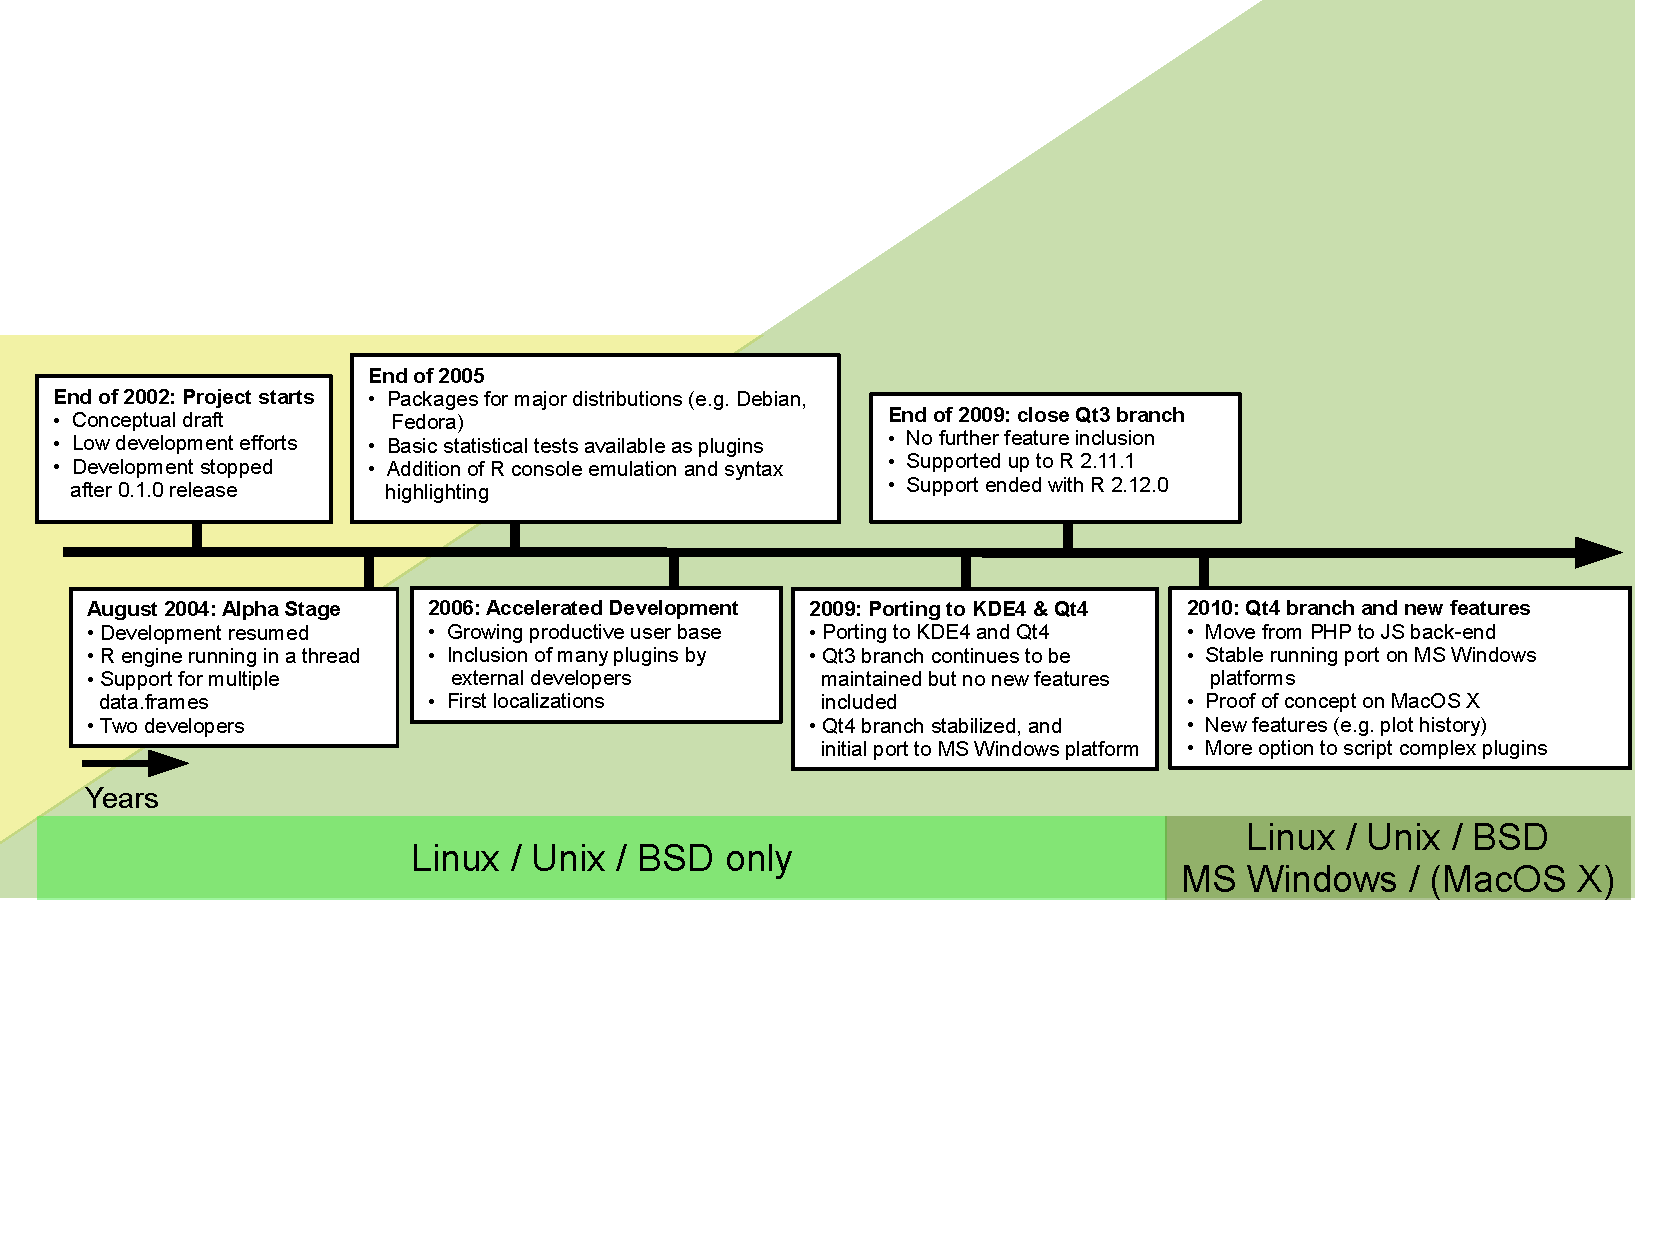
\includegraphics[clip=true,trim=0cm 5.7cm 0cm 5.7cm,width=16cm]{../figures/timeline.pdf}
 \caption{Timeline of important development milestones and changes in RKWard.
          Time is presented on an arbitrary scale.}
 \label{fig:timeline}
\end{figure}

The rest of this paper is organized as follows: Section \ref{sec:user_interface} gives an 
overview of the main GUI elements and features of RKWard, followed by a short example 
of a simple RKWard session in Section \ref{sec:using_RKWard}.
Next, Section \ref{sec:technical} discusses some technical aspects of the implementation, comparing them briefly to competing GUI solutions, where appropriate. An example for creating a simple plugin extension to RKWard is shown in Section \ref{sec:example_plugin}.
Finally, some closing comments are made in Section \ref{sec:conclusion_summary}.
